\documentclass[12pt]{book}
\usepackage[width=4.375in, height=7.0in, top=1.0in, papersize={5.5in,8.5in}]{geometry}
\usepackage[dvips]{graphicx}
\usepackage{amsmath}
\usepackage{amssymb}
\usepackage{tipa}
%\usepackage{txfonts}
\usepackage{textcomp}
%\usepackage{amsthm}
%\usepackage{array}
%\usepackage{xy}
\usepackage{fancyhdr}

\pagestyle{fancy}
\renewcommand{\chaptermark}[1]{\markboth{#1}{}}
\renewcommand{\sectionmark}[1]{\markright{\thesection\ #1}}
\fancyhf{}
\fancyhead[LE,RO]{\bfseries\thepage}
\fancyhead[LO]{\bfseries\rightmark}
\fancyhead[RE]{\bfseries\leftmark}
\renewcommand{\headrulewidth}{0.5pt}
\renewcommand{\footrulewidth}{0pt}
\addtolength{\headheight}{0.5pt}
\setlength{\footskip}{0in}
\renewcommand{\footruleskip}{0pt}
\fancypagestyle{plain}{%
\fancyhead{}
\renewcommand{\headrulewidth}{0pt}
}
%
%\parindent 0in
\parskip 0.05in
%
\begin{document}
\frontmatter
\pagestyle{empty}
%\pagenumbering{}
% Set book title
\title{\textbf{A course on Quality of Service (QoS)}}
% Include Author name and Copyright holder name
\author{Jaume Barcelo}
% 1st page for the Title
%-------------------------------------------------------------------------------
\maketitle
%
\pagestyle{fancy}
%
\tableofcontents
%
\mainmatter
%
\chapter{About the course}

\section{Course Data}

Code: 21738

Course name: ``Protocols de qualitat de servei en xarxes''

Teacher: Jaume Barcelo

Credits: 4

Year: 3rd year

Trimester: Spring

\section{Introduction}
This is a course on Quality of Service in data networks, which is usually abbreviated as QoS.
QoS is about discriminating traffic.
It is about favouring some data packets at the expense of others.
The name can be misleading, as one might think that all packets are benefited from the implementation of QoS.
This is not the case.

A good parallelism to understand QoS is road traffic.
There are some vehicles (typically police, ambulance and firefighters) that receive priority over the others. 
This is not perceived as something negative, as this vehicles incur in tasks that are more important or urgent than the average vehicle.

This parallelism is very illustrative to convey the idea, that QoS does not make the road wider, it simply prioritizes some traffic.

At some point, networks engineers may face the dilemma of investing their efforts and money in either implementing QoS (prioritizing traffic) or increasing the available bandwidth (making the road wider).
The latter option has the advantage that it benefits all the traffic of the network.
Ideally, if the bandwidth is sufficiently over-provisioned, the packets never have to wait in the routers queues.
In the road analogy, if the roads are wide enough, there are never traffic jams.

Unfortunately, making the roads wider or the networks faster does not always solve the problem.
As the users perceive that there is plenty of bandwidth available, they might decide to put it a better use by downloading collections of movies that they will never have time to see.
There is nothing wrong with downloading collections of movies, but the sheer volumes of data may fill up the queues and introduce unacceptable delay and jitter in VoIP calls.

And why is this a problem? Well, at some point network engineers that deploying separate networks for each service represented too much work (and money).
From an engineering and economic point of view, it is much more advantageous to offer the different services on a single network.
It is common nowadays that telephony, video-conference, web, remote backup and file sharing services share the same network.
The term to refer to these networks that support various services is ``converged networks''.
The only problem is that the different services have totally different requirements with regards to required bandwidth and delay.

The service that consume a large amount of bandwidth and do not have strict delay requirements can easily create a ``traffic jam'' that prevents the offering of services with low delay requirements that consume very little amount of bandwidth.
Obviously, it is still possible to offer the two kinds of service simultaneously if we implement QoS mechanisms that prioritizes the low delay traffic.

QoS is a controversial topic.
Net neutrality, which is related to QoS is even more controversial \cite{bachula2006}.
Nevertheless, QoS (or ``bandwidth management'') has been used by ISPs in practice \cite{cooper2011bum}.
We will try to cover the subject from a neutral point of view and you, equipped with the knowledge of the course, will take your own decision about the usefulness of QoS.

The course is divided in three conceptually different parts: lectures, seminars and lab assignments.
In lectures I will introduce you to the nuts and bolts of QoS.
In the seminars, we will review the concepts of queueing theory covered in previous courses, and extend them to consider different traffic classes.
In the lab assignments you will implement some QoS tools and, when possible, validate them with the methods studied in the seminars.

\section{Syllabus}
\begin{itemize}
  \item Lectures
  \begin{enumerate}
    \item Introduction to QoS
    \item QoS Requirements
    \item QoS Service Level Agreements
    \item QoS Mechanics
    \item QoS Architectures
    \item Deploying Diffserv
    \item Capacity Admission Control
    \item SLA and Network Monitoring
    \item Core Capacity and Traffic Engineering
  \end{enumerate}
  \item Seminars
  \begin{enumerate}
    \item Review of basic concepts. Exponential distribution. Poisson Traffic. Little's Theorem. PASTA theorem.
    \item Delay in a network interface with Poisson arrivals, a single (finite) buffer and exponential transmission time.
    \item Delay in a network interface with Poisson arrivals, two traffic classes and exponential transmission time. Preemptive priority and non-preemptive priority.
    \item Delay in a network interface with a general transmission time. Priority queueing in a network with a general transmission time.
  \end{enumerate}
\item Lab Assignments
  \begin{enumerate}
    \item Program a UDP Poisson traffic generator and a traffic sink capable of computing delay (min/avg/max). Packet drop should also be measured.
    \item Program a packet buffer. It should support both exponential and deterministic transmission time. The buffer size is taken as a parameter and it may be infinite.
    \item Program a buffer that implements priority queueing. It should support both exponential and deterministic transmission time. The buffer size is taken as a parameter and it may be infinite.
    \item Implement a QoS tool of your choice: policer, token bucket, leaky bucket.
    \item Combine the different QoS elements that you and your classmates have programmed in a QoS enabled network. Invent an scenario, describe the requirements and explain how your solution addresses such requirements.
  \end{enumerate}
\end{itemize}

\section{Bibliography}

The lecture closely follow the book:

John Evans, Clarence Filsfils ``Deploying IP and MPLS QoS for Multiservice Networks''.

\section{Evaluation Criteria}

The grading is distributed as follows:
\begin{itemize}
\item Lectures continuous assessment, 10\%
\item Seminars continuous assessment, 10\%
\item Blackboard problem solving, 10\%
\item Lab assignments, 10\%
\item Individual continuous assessment quiz, 10\%
\item Final exam, 50\% (Possibility of re-take exam)
\end{itemize}

It is necessary to obtain a decent mark (4 out of 10 or 20 out of 50) in all the different evaluation aspects.
To pass the course, 50 out of the total 100 points need to be obtained.

\section{Survival guide}

\subsection{How to pass the course}

Statistically speaking, you will pass the course if you do all the following:
\begin{itemize}
\item Attend lectures, participate and ask questions.
\item Attend seminars, try to solve the problems on your own and discuss them in small groups.
\item Volunteer to solve problems on the blackboard.
\item Attend labs and use lab time to solve the lab assignments.
\item Participate in the planning and coding of the labs assignments. Read carefully the code of other team members and make sure you understand it and can explain it to others.
\item Study for the continuous assessment quiz, as it is a warming up exercise to face the final exams with success guarantees.
\end{itemize}

\subsection{Continuous Assessment}
In this course we implement continuous assessment.
This means that if you work hard from day zero, the course will be pain-free.

Continuous assessment includes multiple-choice quizzes in lectures and seminars.
You also have to write reports in labs (one for each group).
The source code and the report for the labs is submitted via moodle.
Remember to write always your name and NIA in all the material you hand in or upload to moodle. 
You also have to include you name and NIA in all the source code files you send me.

There is not a template for the report.
I recommend describing key design and implementation aspects, clarifying possible deviations or improvements on the initial assignment, and including examples.
The example should include the input commands as well as the output results.
The report and the code will be submitted at the end of the class via moodle.
At the beginning of the next class, you will have to demonstrate that your programs actually work.

\subsection{Collaboration Policy}
You are encouraged to collaborate with other students in the resolution of problems and assignments.
However, you should firs try to solve it on your own.
Then, you can discuss your solution with others and work together to find a better solution.
Finally, you must ensure that you can solve the problem or assignment alone.

In the labs assignments you will work in teams of three people.
Unless when explicit permission is given to re-use code, each team has to write their own code.

\subsection{Formula Sheet}
This course is not about memorizing equations.
It is about understanding them.
For this reason, you are allowed to use a \emph{formula sheet} in individual tests as long as it fulfills the following requirements:
\begin{itemize}
\item It is a single page (one side).
\item It is handwritten. Your own handwriting.
\item It is delivered together with your answers when the test is finished.
\end{itemize}

\subsection{Questions and doubts}
I like to receive questions and comments.
Normally, the best moment to express a doubt is during the class, as it is likely that many people in the class share the same doubt.
If you feel that you have a question that needs to be discussed privately, we can discuss it right after the class.

\subsection{Continuous feedback}
At the end of the class, I will ask you to anonymously provide some feedback on the course. 
In particular, I always want to know:
\begin{itemize}
\item What is the most interesting thing we have seen in class.
\item What is the most confusing thing in the class.
\item Any other comment you may want to add.

In my previous experience, this information has proven to be invaluable in improving the course, detecting problems at an early stage, and adapting the course to the expectations of the students.

In labs, I will ask each group to hand in a short (few paragraphs) description of the work carried out in class, and the members of the group that have attended the class.
Note that this is different from the lab report, which is the one that it is actually graded.
\end{itemize}

\subsection{How to make you teacher happy}

Avoid speaking while I am talking.
It is not that you cannot talk in class.
You can talk as much as you want when I am silent.
I will make plenty of breaks in which I will ask you to discuss a question with your classmates.
You can also take advantage of the moments in which I erase the blackboard or just scratch my head while staring.
As long as I am not talking, you can talk with your classmates as much as you want.
Obviously, questions are welcome at any time.

\chapter{QoS metrics}
\label{cha:quality_metrics}

If you go to the postal office to submit a packet, you will be offered different options.
In addition to the regular service, it is possible that an urgent service exists.
Probably there is also the possibility sending the packet as certified mail, and some option for delivery notification.
It is likely that there are also special services for packets that are voluminous or heavy.

QoS-enabled packet switched networks also offer different kinds of services for data packet delivery.
In this chapter, we will review the different metrics that are relevant for data networks.
This metrics can be used to establish \emph{service level agreements} (SLAs) which are contracts specifying the QoS expected from a network.
These contracts should also specify how the metrics are actually measured.

As an example, if a network guarantees a delay below 100 ms, it should be specified whether this makes reference to the maximum, the average delay or the 95\% percentile.
The measures will also differ depending whether 5 minutes averages or 1 hour averages are considered.
This makes the specification of SLAs tricky.

\section{Delay}

Delay is the time that it is required to traverse the network from the entry point to the exit point.
Delay is normally considered for real-time services such as voice over IP (VoIP).
The total end-to-end delay is simply the sum of the delay suffered in each of the hops in the data network.
As an example, \ref{fig:four_hops} shows a network with four hops.

\begin{figure}[h]
\centering
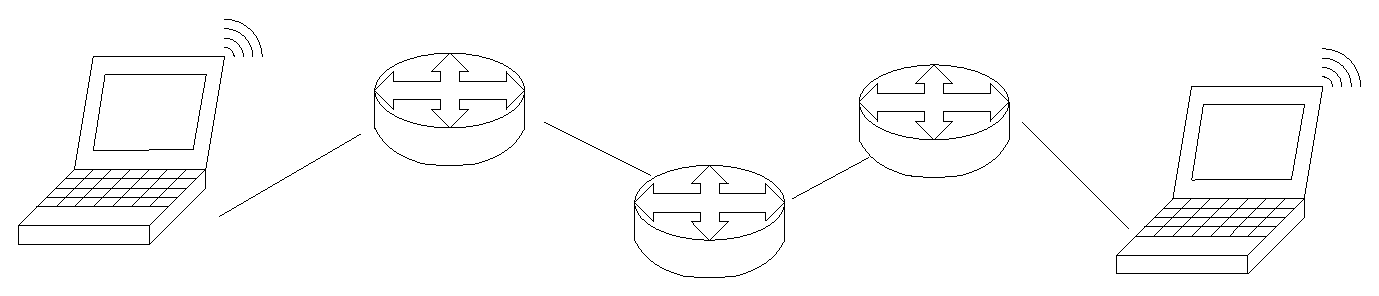
\includegraphics[width=\linewidth]{figures/four_hops.eps}
\caption{A network with two terminals, three routers and four hops.}
\label{fig:four_hops}
\end{figure}

In each hop, there are four different contributions to delay:
\begin{enumerate}
\item Processing: The time required for the router or switching device to put the packet on the outgoing interface queue.
Very short.
\item Queueing: Waiting time on the outgoing interface queue.
Very short if the queue is empty.
\item Transmission: The time required to put the packet on the transmission medium. It is a function of the packet length and transmission rate.
Short in high-speed transmission media.
\item Propagation: The time that it takes for the packet to travel the distance from the hop source to the hop destination.
Short time over short distances. 
And very long when it involves a trip to a geostationary satellite.
\end{enumerate}

\section{Jitter}
Jitter is the variation of delay.
This aspect is specially relevant for real-time and streaming applications.
These applications expect the packets to arrive regularly in time.
As an example, if the encoder application takes a voice stream and splits it into 20 ms chunks that are encoded and sent as packets, the receiver application will expect to receive one packet every 20 ms to reconstruct the voice stream.

If packets are sent every 20 ms but each of them requires a different time to traverse the network, the separation between packets will no longer be 20 ms at the receiving end.
Applications sensitive to jitter use a de-jittering buffer that holds some packets and feeds the decoder at regular intervals.
The packets that suffered a short delay in the network will wait for a longer time in the de-jitter buffer and the packets that suffered a longer delay in the network stay in the buffer for a shorter time.
With this technique, jitter is effectively suppressed at the expense of increasing delay, as shown in figure \ref{fig:dejitter}.

\begin{figure}[h]
\centering
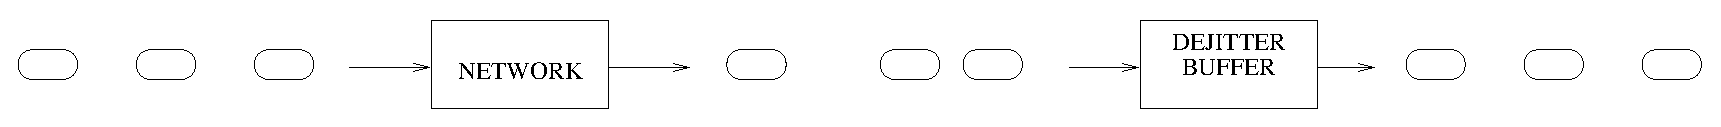
\includegraphics[width=\linewidth]{figures/dejitter.eps}
\caption{The dejitter buffer removes jitter at the expense of adding delay.}
\label{fig:dejitter}
\end{figure}

The de-jitter buffer size in terms of time and packets (or bytes) need to be carefully tuned, to prevent both packet overflow and underflow.
Buffer overflow happens when the buffer is full and cannot accommodate an arriving packet.
Buffer underflow occurs when the decoder asks for a packet and the buffer is empty.

\section{Round Trip Delay}

The round trip delay is the measure of delay used for elastic and interactive applications.
It is the time required for a packet from source to destination and then back to the source again.
You can easily find the round trip delay from your host using the ping command.

\begin{lstlisting}
$ ping www.happyforecast.com
PING happyforecast.com (184.107.100.65) 56(84) bytes of data.
64 bytes from s106.panelboxmanager.com (184.107.100.65): icmp_req=1 ttl=48 time=122 ms
64 bytes from s106.panelboxmanager.com (184.107.100.65): icmp_req=2 ttl=48 time=121 ms
64 bytes from s106.panelboxmanager.com (184.107.100.65): icmp_req=3 ttl=48 time=122 ms
64 bytes from s106.panelboxmanager.com (184.107.100.65): icmp_req=4 ttl=48 time=122 ms
64 bytes from s106.panelboxmanager.com (184.107.100.65): icmp_req=5 ttl=48 time=122 ms
64 bytes from s106.panelboxmanager.com (184.107.100.65): icmp_req=6 ttl=48 time=121 ms
^C
--- happyforecast.com ping statistics ---
6 packets transmitted, 6 received, 0% packet loss, time 5004ms
rtt min/avg/max/mdev = 121.864/122.066/122.181/0.230 ms
\end{lstlisting}

An interactive application (such as web browsing) requires a few round trip delays to complete the dialogue between the client and the server.
Furthermore, the round trip delay also limits how fast the Transfer Control Protocol (TCP) congestion window can grow.
The congestion window grows upon the reception of TCP acknowledgements.
If it takes long for the TCP acks to arrive, the congestion window grows slowly.

In fact, it becomes difficult to take fully advantage of connections with a high \mbox{throughput x delay} product.
These are known as ``long fat pipes'' or ``long fat networks'' (which is shortened as LFN and sometimes pronounced elephant), as explained in RFC 1072 \cite{rfc1072}.

\section{Packet Loss}

The networks may loose some of the packets being sent.
Packet loss has different sources:
\begin{itemize}
\item Physical layer errors. 
The physical layer may flip some of the bits of the packet.
As the packet typically includes some ``cyclic redundancy check'' (CRC), this errors are detected and the whole packet is dropped.
In wireless communications, the occurrence of errors is likely and therefore some additional mechanisms are used.
Forward error correction (FEC) codes can correct some of the errors.
Furthermore, automatic repeat request (ARQ) are used to request retransmission of faulty packets.
\item Queue packet dropping.
In normal network conditions the queue should be almost empty.
However, when the queues start to fill up, it is necessary to discard packets.
Packets can also be discarded preventively, to regulate the pace of TCP flows.
\item Network failure.
Network failure can result in the loss of many packets, depending on the gravity of the failure and the restoration time.
\end{itemize}

From a QoS perspective, it is not only important how many packets are lost, but also the distribution of the loss in the data flow.
As an example consider two networks that loose 10 packets out of 1000. 
The first network looses a packet out of every 100 packets, while the second one looses the 10 packets consecutively. 

A VoIP application using packet loss concealment will be able to hide the packet loss of the first network, but not of the second one.
If a packet voice is lost, the VoIP application can play the trick of playing the previous packet for two consecutive times, and the listener will hardly notice it.
However, the loss of 10 consecutive packets may represent 0.2 seconds worth of audio that are likely to be noticed by the listener.

For a TCP application, the loss of a single packet will result in a quick retransmission.
However, loosing 10 consecutive packets may move the TCP session back to the ``slow start'' mode and substantially reduce the throughput.

\section{Throughput}

Throughput (sometimes also referred to as bandwidth) is the amount of data transmitted per unit of time.
Unfortunately, in practice it may have several different meanings.

It can be related to the line speed, which is the maximum data achieved by the physical medium (e.g, 100 Mbps or 1Gbps).
Some technologies have a variable data rate, such as WiFi, that adapts the transmission speed to channel conditions.
Furthermore, for a given technology, the throughput depends on which is the protocol layer under consideration.
As an example, a 54 Mbps WiFi device is capable of 54Mbps at the PHY layer, but roughly half of that is available at the network layer.
The protocol overhead decrease the throughput as we move up the layer stack.

Quite often the term throughput refers to the amount of data per unit of time that it is actually sent, not at the capabilities of the network.
Or it may refer to the amount of throughput that has been contracted to the Internet Service Provider (ISP).
It was common to define this contracts in terms of ``committed information rate'' (CIR) that the ISP promised to carry, and the ``peak information rate'' (PIR) that the ISP would carry if it was possible.
This throughput could be measured using ``token buckets'' that allow for some burstiness. 

Another interesting concept is the 95th percentile billing, which is the kind of contract between ISPs and heavy traffic consumers/producers.
In this contract there is a commit (or baseline speed) for a given price (say 20 Mbps for 180 Euro).
The throughput consumption is measured in 5 minutes averages, and the 95th percentile value is considered.
Then, if the 95th percentile is higher than the committed rate, the customer has to pay extra fee for each Mbps exceeding the committed rate (e.g., 10 Euro per additional Mbps).

The ISP normally have different kind of offers the user can choose from, depending on the predicted user consumption.
For example, the same ISP considered in the previous paragraph might have an offer of 40 Mbps for 300 Eur plus 5 Eur for additional Mbps.
\section{Packet re-ordering}

Many applications need that the packets are received in the same order than they are sent.
To this end, TCP re-orders packets and doesn't offer the data to the upper layers if there are gaps in the data flow.
Similarly, in a VoIP application the voice packets should be handled to the decoder in order.

It is a desirable property of the networks that they maintain packet ordering.
A basic principle is to assign packets belonging to the same flow to the same queue.
In case of a router that performs load balancing among different links, a hash of the source/destination ip address/port can be used to decide the path of the packet, to make sure that all packets of the same flow follow the same path.

\section{Availability}

High availability is a critical issue for data networks.
It is often said that ``five nines'' or 99.999\% is required from carrier grade networks.
This means 5.26 minutes of (non-scheduled) downtime per year.

Some common metrics in terms of availability are the mean time between failures (MTBF) and the mean time to restore (MTTR).
The availability can then be computed as $Availabilty = \frac{MTBF}{MTBF+MTTR}$.

Given a system which is composed of several subsystems either in ``series'' or in ``parallel'', it is possible to compute the system overall availability.
In ``series'' means that the system works only when all subsystems are working, and in ``parallel'' means that the system fails only when all subsystems fail.

\section{Application requirements}
Broadly speaking, we can classify the applications in two different kinds: inelastic (or real-time) and elastic (non-real time).
An example of an inelastic application is VoIP and an example of an elastic one is remote backup.

Inelastic applications have a given throughput (and delay) requirements and are not flexible at all about this.
As an example, if an streaming service requires 2Mbps, it will not work with 1.5 Mbits.
The good part of the inelastic applications is that they only consume what they require.
Using the same example streaming application, it will use only 2 Mbps even if there is more available.

On the other side, elastic applications are more flexible about their requirements.
If a backup service has only 1.5 Mbps available instead of 2 Mbps, the backup will take longer to complete that this is not typically a problem.
Another characteristic of elastic applications is that they are often greedy, which means that they will take as much throughput as it is available.
In this attempt to reach the limits of throughput availability, they create some temporary congestion or queue build up that is detrimental to real time services.

Somewhere in between real time and non real time applications we find interactive applications. 
They don't have the tight throughput and delay constraints of real time applications, but still they have to be responsive for the user to enjoy the experience.
Examples of interactive applications are web browsing, Internet messaging.

\subsection{VoIP}
It has tight delay constraints (below 200ms) and does not consume too much throughput (around 100 Kbps per flow).
As delay grows, conversation seems more artificial as there is the sensation that the other party is not responding.
The human conversation protocols break down and it can be irritating.
It is also unpleasant if there are noise and artifacts that make it difficult to understand the conversation, and for this reason packet loss has to be very low.

A as a target reference, packet loss should be kept below 1\%.

\subsection{Videoconference}
The requirements for voice are the same as for VoIP.
Regarding the video, it requires more throughput but the quality is usually not that important.
Users don't get too annoyed if the image freezes for half a second, as long as the voice quality is fine.

\subsection{Streaming}
It requires a lot of throughput and the display quality is important.
The advantage is that it is possible for the receiver to have a buffer to partially alleviate jitter or even packet loss if retransmission is possible.

\subsection{Video on demand}
In this case the, the buffer can be larger as the content is pre-recorded and it is not critical to show it in real-time.

\subsection{Web browsing}
In principle, the load placed by web browsing is low and the delay requirements are mild (a few hundreds of milliseconds is not a problem). 
However, as the video on the web gains popularity, the throughput requirements are larger and get closer to those of Video on demand.

\subsection{Peer to peer file exchange and remote backup}
This may involve the transmission of massive amounts of data.
The advantage is that they can often be delayed and accommodated in off-peak hours.

\subsection{Gaming}
Real time online gaming requires short delays.
Normally the volume of data exchanged is low.

\section{Service Level Agreements}

A company owning different networks at different locations normally pays an Internet Service Provider (ISP) for connectivity among those networks.
The ISP offers different services that are labelled with marketing names such as gold, silver and bronze.
Each service has different characteristics in terms of QoS metrics.

The company has to take the decision to take one or more of those services according to the applications that are needed.
Typically, for VoIP applications, the highest QoS (gold) is needed.
Other applications such as nightly backup may use other services that allow to transfer high volumes of data at low rates (bronze).

Besides the QoS commitments, it is common to include in the contract a Committed Information Rate (CIR) and Peak Information Rate (PIR).
The ISP provides QoS guarantees for the traffic which is below the CIR, and allows rates up to the PIR with no QoS guarantees.
As an example, traffic over the CIR and below the PIR may be discarded in case of congestion.

To be more specific, the agreement includes not only a rate, but also a depth of a token bucket, which is a measure of the burstiness of the traffic. 
Token buckets will be covered in more detail in the next chapter.

\subsection{95\% percentile billing}

An alternative of the CIR/PIR approach is the 95\% percentile billing.
The client commits to a given data rate.
Then, the actual traffic is measured in averages of 5 minutes.
The measure that is used for billing is the one that occupies the 95\% percentile.
That means that 95\% of the measures are lower that this value and only the 5\% are higher (peaks).

If the measured 95\% percentile is higher than the committed rate, the client has to pay a penalty that is specified in the SLA.
For example, 10 Euro for each Gbps in excess of the committed rate.

\backmatter
%
\bibliographystyle{plain}
\bibliography{rfc,my_bib}
\end{document}
